\pdfoutput=1
\begin{figure}[tb!]
    \centering
    \begin{subfigure}[b]{1.0\linewidth}
        \centering
        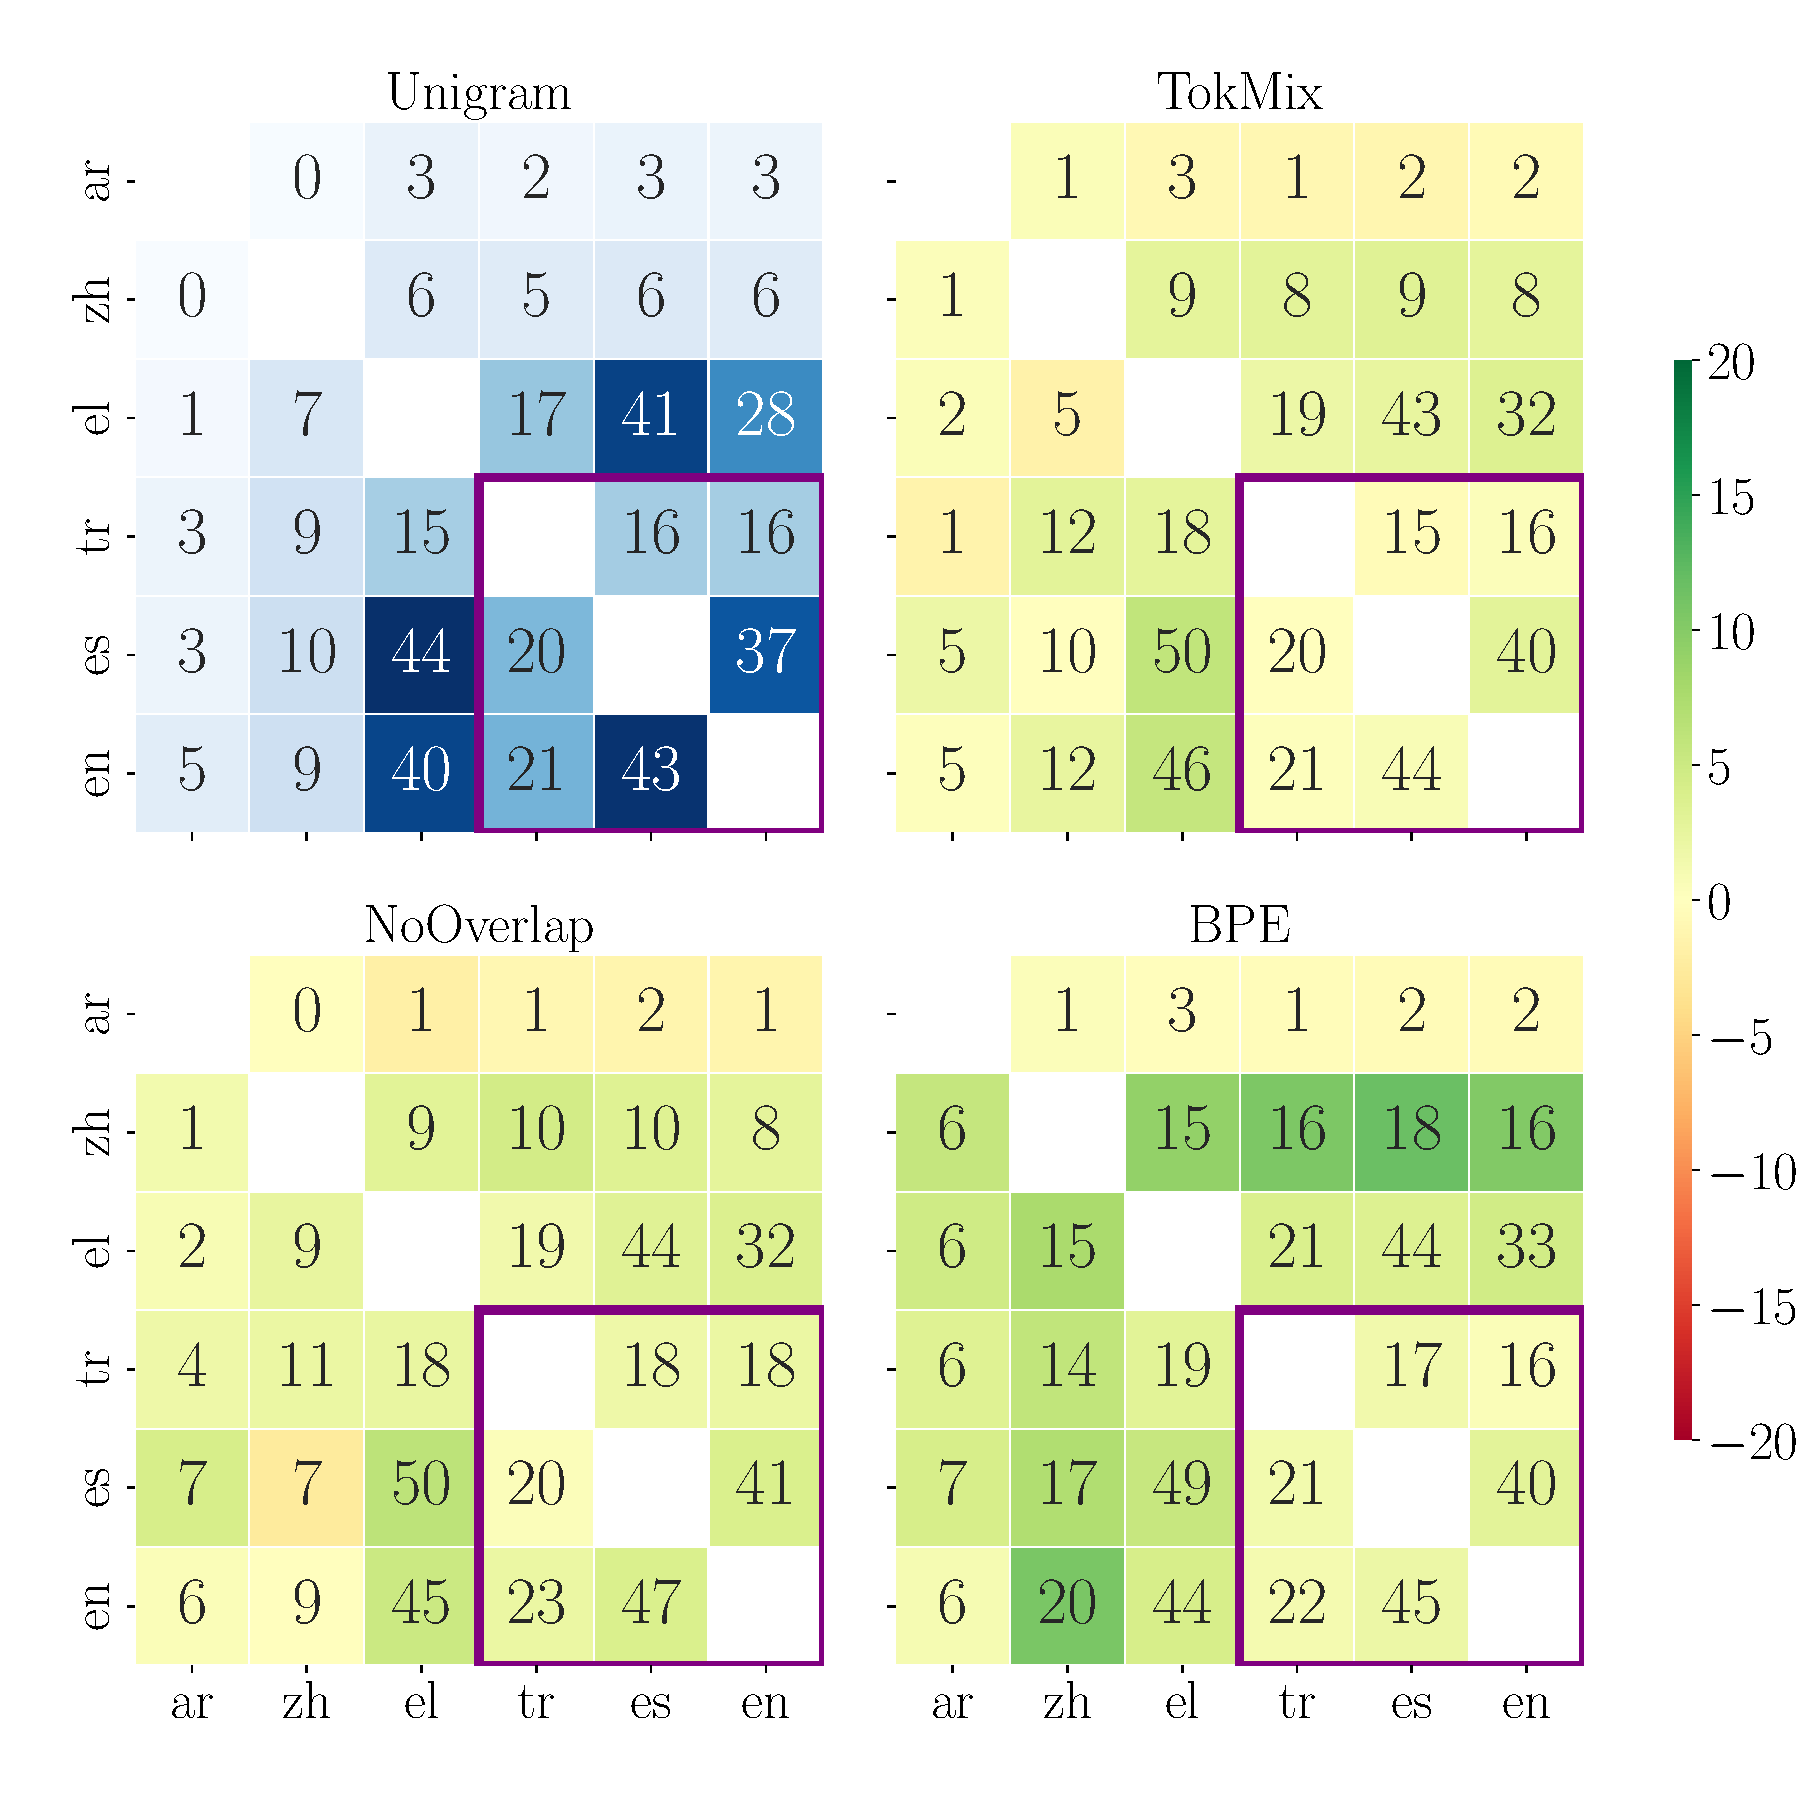
\includegraphics[width=0.9\linewidth]{figures/UD_F1_transfer_.pdf}

        \caption{Dependency labeling}
        \label{fig:ud_transfer}
    \end{subfigure}
    \begin{subfigure}[b]{1.0\linewidth}
        \centering
        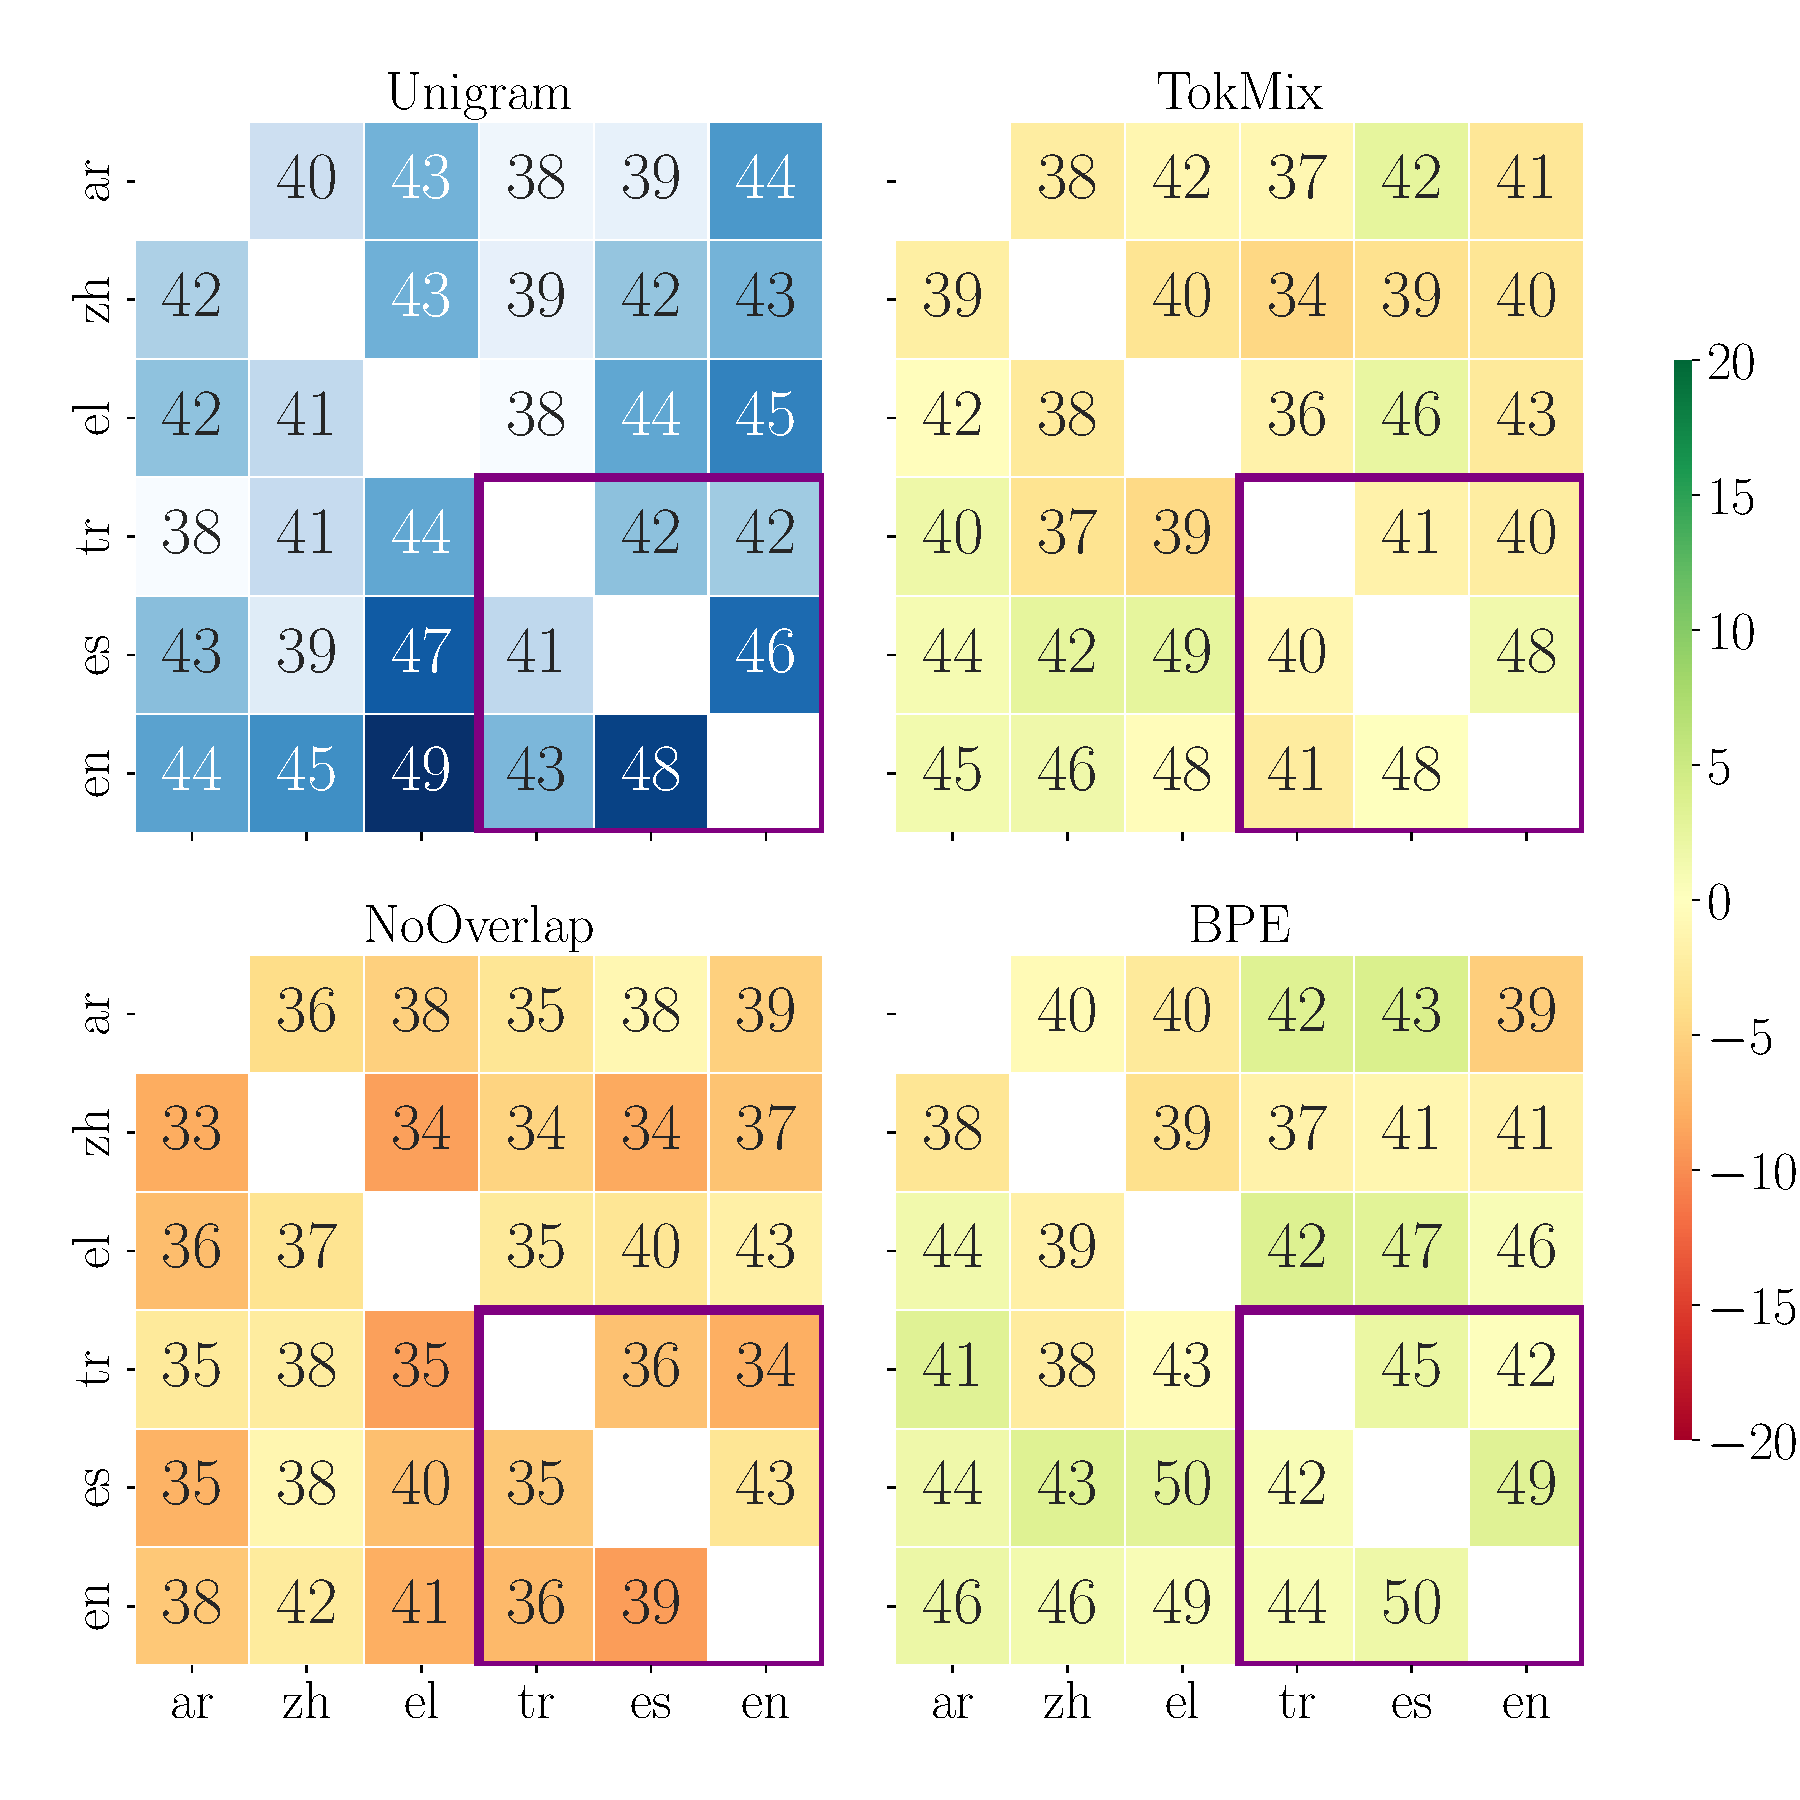
\includegraphics[width=0.9\linewidth]{figures/XNLI_Acc_transfer_.pdf}
        
        \caption{Natural Language Inference}
        \label{fig:xnli_transfer}
    \end{subfigure}
    \begin{subfigure}[b]{1.0\linewidth}
        \centering
        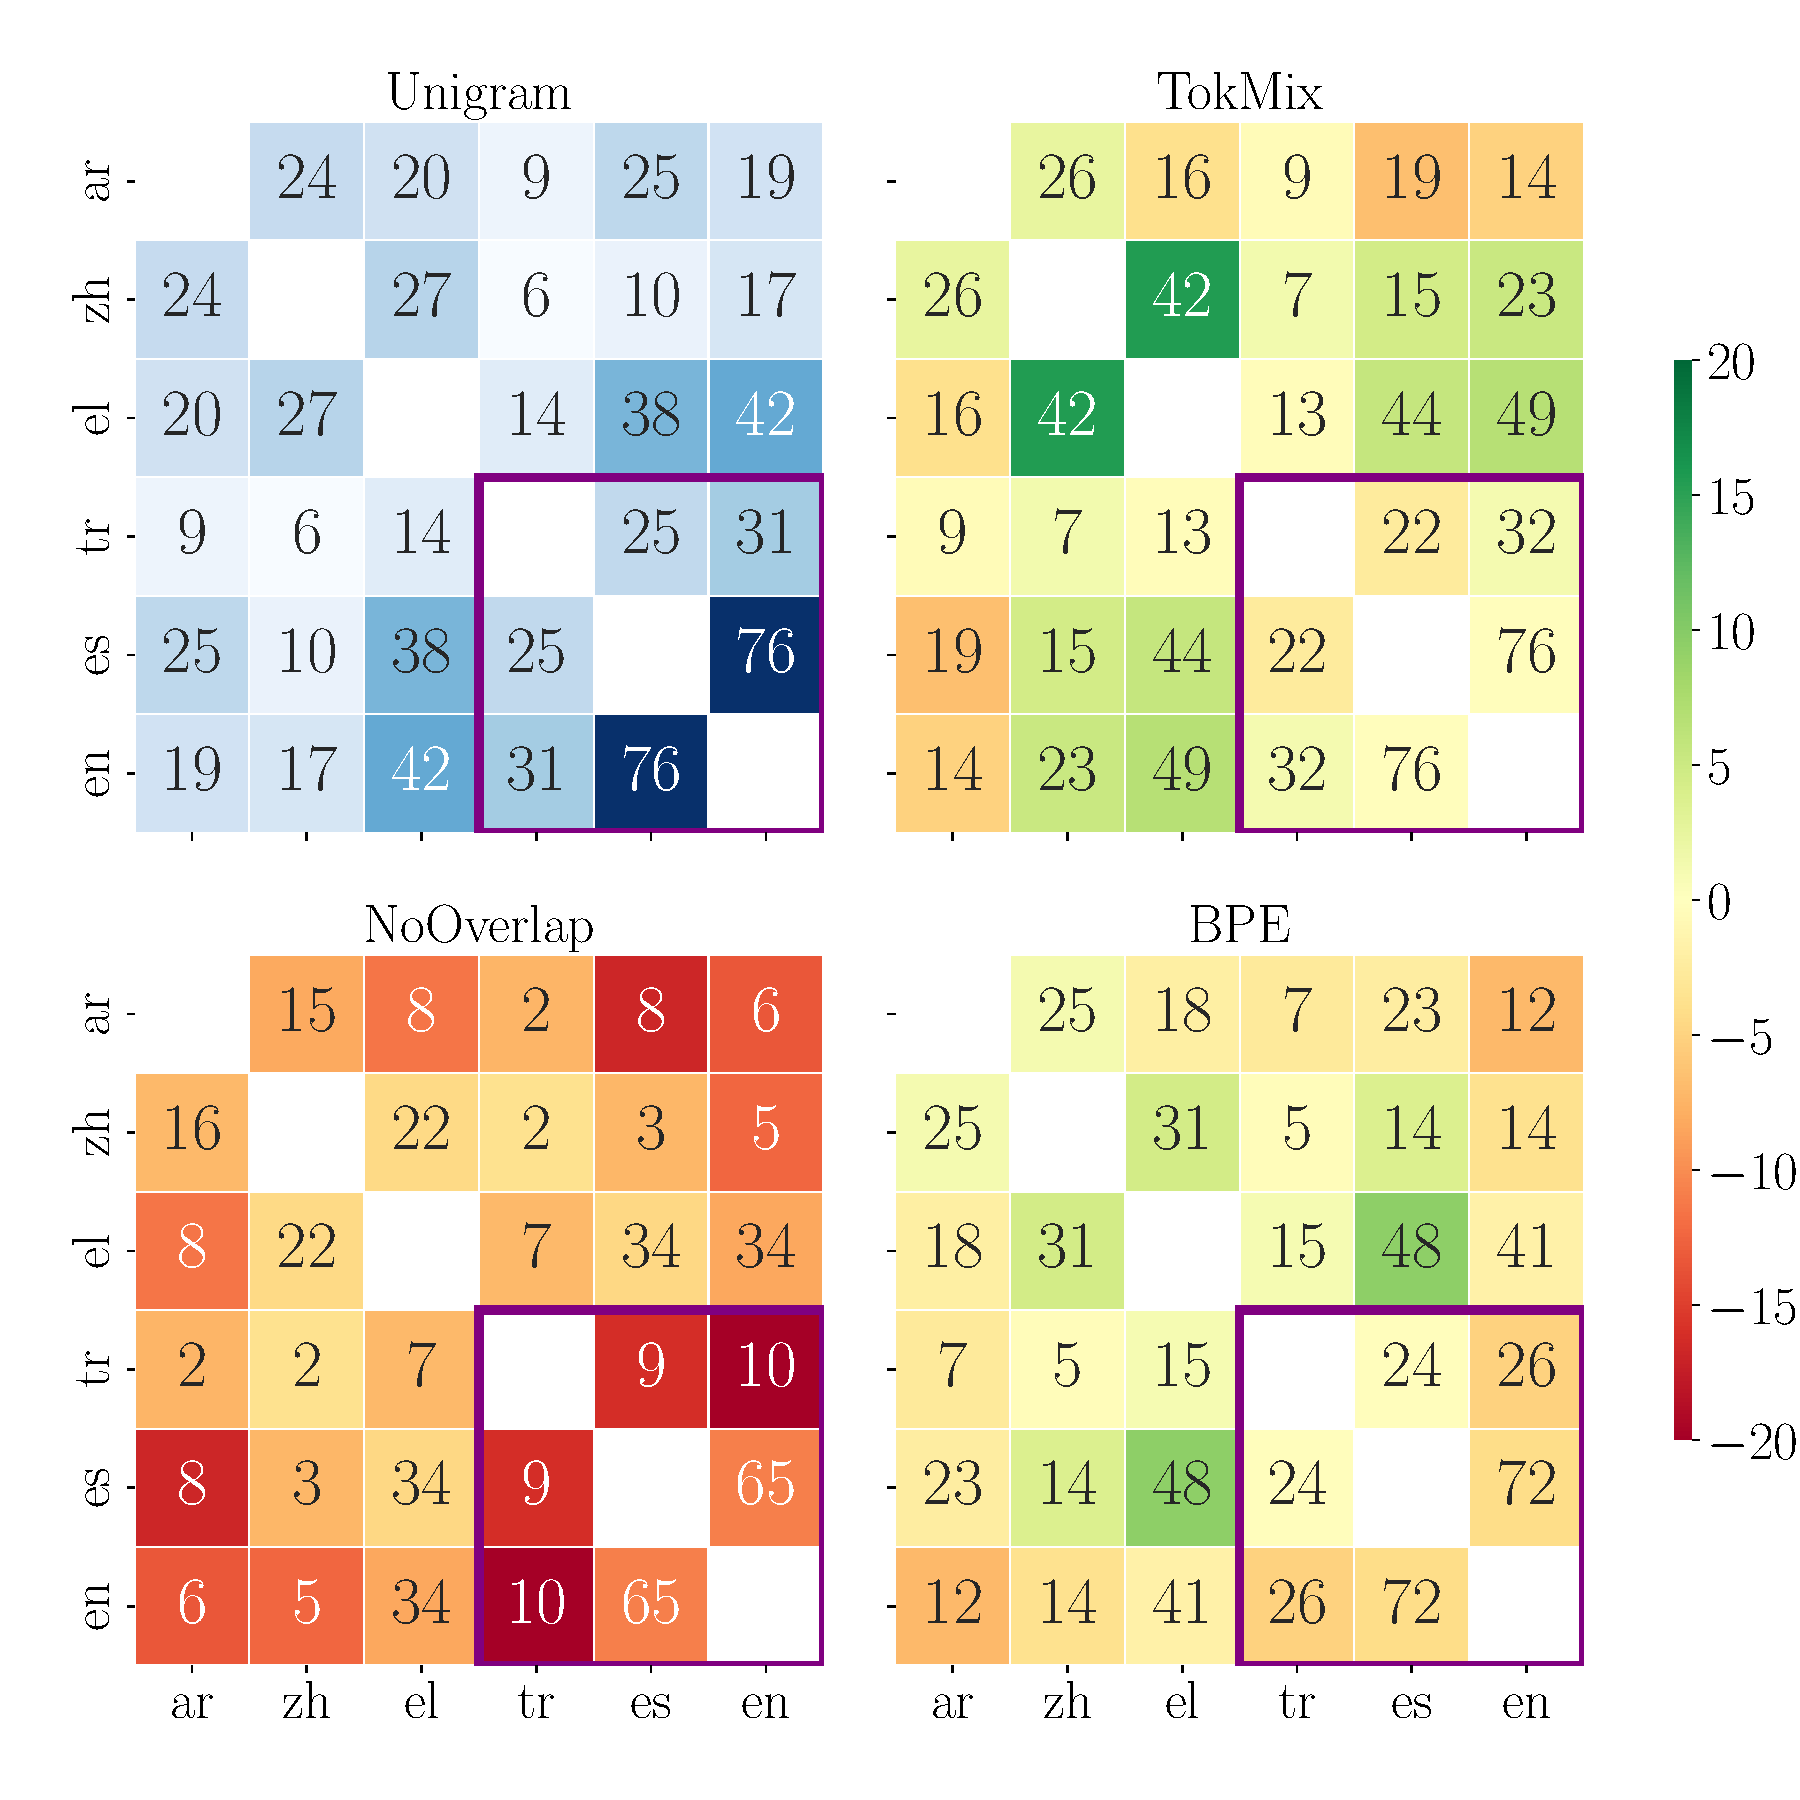
\includegraphics[width=0.9\linewidth]{figures/Tatoeba_Acc_transfer_.pdf}
        
        \caption{Sentence retrieval}
        \label{fig:tatoeba_transfer}
    \end{subfigure}
    \caption{The rest of the 6-language cross-lingual transfer results. The absolute values are presented for the Unigram tokenizer. For other tokenization methods, we show  the difference from the unigram algorithm.}
\end{figure}
